\chapter{Path Names}
\label{pathnames}

\section{Absolute Paths}

Imagine your file hierarchy as a map, where folders represents streets and files represent houses, as in Figure~\ref{fig.files}.

\begin{figure}[!ht]
\begin{center}
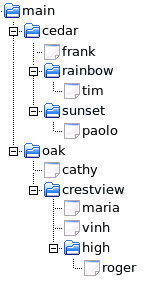
\includegraphics[width=0.2\textwidth]{figs/streets.png}
\caption{A Tree of Directories and Files}
\label{fig.files}
\end{center}
\end{figure}

An absolute pathname is like giving directions starting at the very outside of the map and working inwards. The directions for getting to Maria's house in an absolute fashion would be ``Start at Main street, then go to Oak street, then to Crestview Drive, and there is Maria's house.'' In terms of Linux or Mac OS pathnames, that would be \texttt{/main/oak/crestview/maria}.

In Linux and Mac OS, the / (slash) separates levels of directory. The topmost level of the file system has no name, so when you start from the topmost level, you start with a separator---the slash.

The absolute pathname to get to Frank's house is ``Start at Main Street, go to Cedar Street, and there is Frank's house.'' (\texttt{/main/cedar/frank}).

On Windows, if all these files were on the \texttt{C:} drive, the absolute path would be \texttt{C:\textbackslash main\textbackslash cedar\textbackslash frank}.

\section{Relative Paths}

Now let's say you were on Crestview Drive in front of Maria's house and someone asked you how to get to Vinh's house. You wouldn't answer, ``Start at Main Street, then go to Oak Street, then go to Crestview Drive...'' You wouldn't do that because you're already on the correct street. You would just say ``Vinh's house is next door.'' That is a {\em relative pathname}---starting from where you are right now, how do you get to the destination? When specifying a Java path, if you are in directory \texttt{/main/oak/crestview}, the relative filename for file \texttt{vinh} is just that: \texttt{vinh}, because it is in your current directory.

If you were on Cedar Street and someone asked you how to get to Tim's house, you would tell them to go to Rainbow Drive, and there's Tim's house. The relative path is \texttt{rainbow/tim}. On Linux or Mac OS, relative pathnames {\em never} begin with a slash; on Windows they {\em never} begin with a drive name.

If you were on Oak Street and someone asked you how to get to High Street, you would answer with a relative path: Go to Crestview Drive, and from there to High Street. As a relative path, that's \texttt{crestview/high}.

Now comes a tricky one. You're on Sunset Drive (in the diagram, that is the vertical dotted line beneath the folder labeled \texttt{sunset}), and someone asks you how to get to Frank's house. You have to say: ``Go back up one street (that puts you on Cedar street, the vertical dotted line under the \texttt{cedar} folder); that's where you will find Frank's house.'' Whenever you tell someone to go back up one level in the file hierarchy, you use two dots \texttt{..} to symbolize the parent directory. In Linux terms, the relative pathname is \texttt{../frank}

Important: The relative pathname is not \texttt{cedar/frank}. If you are on Sunset Drive, you can't go directly to Cedar Street; it's not one of your sub-directories.

Using \texttt{../cedar/frank} is also incorrect. That would mean ``back up one level (which puts you on Cedar street) and then go to Cedar street (but you can't; inside the \texttt{cedar} folder there is no other folder named \texttt{cedar}!)

You can use \texttt{..} as often as you need to in a relative path. If you are on Rainbow Drive and want to go to Cathy's house, you have to back up to Cedar Street, and from there back up to Main Street. Once there, you have a straight shot to Oak Street and Cathy's house. Thus, the relative path is \texttt{../../oak/cathy}

There is one other abbreviation you can use in Java paths: the dot \texttt{.} means ``my current directory,'' so if you were to use the path \texttt{./example.txt}, it would be a relative path name to the file \texttt{example.txt} in the current directory, exactly the same as \texttt{example.txt}. This seems redundant, but the ``my current directory'' concept is often convenient when using the command line interface in Mac OS or Linux. 
